
  
\documentclass[letterpaper, 12pt]{article}

\usepackage{natbib}
\usepackage{hyperref}
\usepackage{graphicx}
\usepackage{amsmath}
\usepackage[dvipsnames]{xcolor}
\usepackage[format=plain,justification=RaggedRight, labelfont=bf]{caption}
\usepackage[style=plain,floatrowsep=qquad]{floatrow}
\usepackage{sectsty}
\usepackage[compact]{titlesec}
\usepackage{aas_macros}
\usepackage{amsmath}
\usepackage[charter]{mathdesign}
\usepackage[margin=1in]{geometry}
\usepackage{fancyhdr}
\usepackage{float}
\pagestyle{fancyplain}
\renewcommand{\headrulewidth}{0pt}
\lhead{}
\chead{}
\rhead{}
\lfoot{}
\cfoot{\thepage}
\rfoot{}

\hypersetup{pdfpagemode={UseOutlines},
  bookmarksopen,
  colorlinks,
  linkcolor={Black},
  citecolor={Black},
  urlcolor={RoyalBlue}}

\bibliographystyle{apj}

\newcommand*{\eg}{{e.\,g.,}\xspace}
\newcommand*{\ie}{{i.\,e.,}\xspace}

\newcommand{\todo}[1]{{\color{red} TODO: #1}}

%%%%%%%%%%%%%%%%%%%%%%%%%%%%%%%%%%%%%%%%%%%%%%%%%%%%%%%%%%%%%%%%%%%%%%%%%%%%%%%%

% Alter some LaTeX defaults for better treatment of figures:
% See p.105 of "TeX Unbound" for suggested values.
% See pp. 199-200 of Lamport's "LaTeX" book for details.
% General parameters, for ALL pages:
%\renewcommand{\topfraction}{0.9}    % max fraction of floats at top
%\renewcommand{\bottomfraction}{0.8} % max fraction of floats at bottom
%
% Parameters for TEXT pages (not float pages):
\setcounter{topnumber}{2}
\setcounter{bottomnumber}{2}
\setcounter{totalnumber}{2}             % 2 may work better
\setcounter{dbltopnumber}{2}            % for 2-column pages
\renewcommand{\dbltopfraction}{0.9} % fit big float above 2-col. text
\renewcommand{\textfraction}{0.07}  % allow minimal text w. figs
%
% Parameters for FLOAT pages (not text pages):
\renewcommand{\floatpagefraction}{0.7}  % require fuller float pages
%
% N.B.: floatpagefraction MUST be less than topfraction !!
\renewcommand{\dblfloatpagefraction}{0.7} % require fuller float pages


\begin{document}
\author{Corey Brummel-Smith}
\title{Title}

\section{Introduction}

The elements that comprise everything we see around us, in fact, nearly everything from the second row of the periodic table down, didn't exist before the formation of the first stars. Understanding the first stars is not just important for understanding our cosmic origins; they're crucial in understanding the formation of galaxies throughout cosmic time, and the evolution of the early universe as a whole. The difficulty is, even when we look deep into the sky, far back in time, all these first stars are too faint or already dead, so studying them observationally is not currently possible. The only connection we have to them are the clues they've imprinted on the second generation of stars, by enriching them with their metals. When these, so-called, Population III (Pop III) stars explode, they enrich the environment with metals formed in their supernovae, and the remnants can later collapse to form new, metal-poor (Pop II) stars \citep{Chiaki2019}. These stars can have much longer lives and may still exist today in places like the galactic halo and ultra-faint dwarf galaxies (UFDGs) \citep{Kirby2008}. One of the goals of stellar archeology is to infer the properties of the first stars by observing the distribution and metallicities of their long-lived descendants. However, since individual Pop II stars may be enriched by multiple Pop III progenitors, it is often impossible to infer the precise masses and metallicities of the first stars. We will address this problem with two separate types of numerical simulations. Each type of simulation will provide a unique connection between Pop III and Pop II stars. In the first project, we will investigate whether supernova induced star formation can produce second-generation, metal-poor stars enriched by a single progenitor. In the second project, we will track metals from multiple Pop III stars in cosmological simulations, and determine exactly how many Pop III stars enrich the second-generation stars. \textbf{Ultimately, this work will provide a deeper understanding of the transition away from a metal-free universe, and allow us to constrain the masses, metallicities, and distribution of the first stars.}

\subsection*{Carbon Enhanced Metal-Poor Stars}

In some cases, the metallicity of the second stars is set entirely by the yields of the Pop III stars. The stellar life-cycle produces more metals with each successive generation, and thus, today, we see stars with a metal abundance orders of magnitude larger than that of the stars in the early universe. Since the metal abundance of the universe continually grows over time, metallicity is a good indicator of the age of a system. This is why low metallicity stars are the best places to study the chemical composition of the early universe and the first stars. Because of their low metallicity and old age, carbon-enhanced metal-poor (CEMP) stars are of particular interest in stellar archeology. These stars are divided into three groups based on their iron and carbon abundances. Group II and III stars have lower metallicity than Group I, and are comprised of CEMP-no stars, which are CEMP stars with no overabundance of s-process elements \citep{Maeder2015}. 

CEMP-no stars are of particular interest to us because detailed analysis of their chemical composition strongly supports the hypothesis that the pre-stellar clouds in which these stars formed, were enriched by the first-generation stars \citep{Yoon2016}. However the details of their formation and their connection to the first stars is not fully understood. \cite{Yoon2016} also point out that more than one class of progenitors for Group II and Group III stars exist, and yet-to-be suggested sites of star formation and metal enrichment may account for the contrasts between Group II and III. \textbf{In our first project, we will investigate a new formation channel, fueled by triggered star formation, that could help explain the origins and differences between Group II and Group III CEMP-no stars. In project 2, we will investigate whether these differences arise from the number of Pop III progenitors.}


\section{Proposed Work}
The overall goal of our two projects will be to use numerical simulations to track metals from individual population III stars from their supernova remnants, all the way to their final resting place in the stellar nurseries of the second-generation stars. These simulations will provide a quantitative connection between the first stars and their metal-poor descendants, which will allow us to determine the properties of actual Pop III stars, from observations of CEMP stars and the metal-poor galaxies in which they live. In project 1, we will perform supernova induced star formation simulations to determine the properties of stars that form from a single Pop III progenitor. In project 2, we will use cosmological simulations to study how multiple Pop III progenitors seed the formation of the second stars.

\subsection*{Project 1: Supernova Induced Formation of the Second Stars}
\label{sec:tsf}

\textbf{Motivation:} We know from simulations, a typical formation channel for the second-generation stars is the internal enrichment (IE) scenario \citep{Chiaki2019}. IE occurs when a Pop III star explodes, enriching its host dark matter halo with metals, and the metal-enriched supernova remnant re-collapses to form new stars. This process occurs on a timescale of several tens of Myr, which is much longer than the lives of massive Pop III stars. For reference, a 40 $M_\odot$ Pop III star has a main sequence lifetime of 3.86 Myr \citep{Schaerer2002}, much shorter than the timescale of supernova remnant re-collapse. This means it is possible and -- maybe even likely -- that Pop II stars will be seeded by multiple Pop III progenitors, making it difficult to infer the metal yields and masses of the individual Pop III stars. However, if all the metals in a cluster of Pop II stars were to come from a single progenitor, one could infer the yields and mass of the progenitor by measuring the metallicity of the cluster. Enrichment by a single progenitor could happen by triggered star formation. If a Pop III star explodes in close proximity to a molecular cloud, it could mechanically crush it into gravitational collapse, or heat the surrounding environment enough for the increased pressure to induce gravitational instability. A diagram of this is shown in figure \ref{fig:tsf}. After the cloud becomes gravitationally unstable, stars will form in roughly the free-fall time of the cloud. This would typically be on the order of millions of years rather than several tens of millions. Therefore, there would not be enough time for other Pop III stars to contaminate the protostellar cloud.

\begin{figure}
  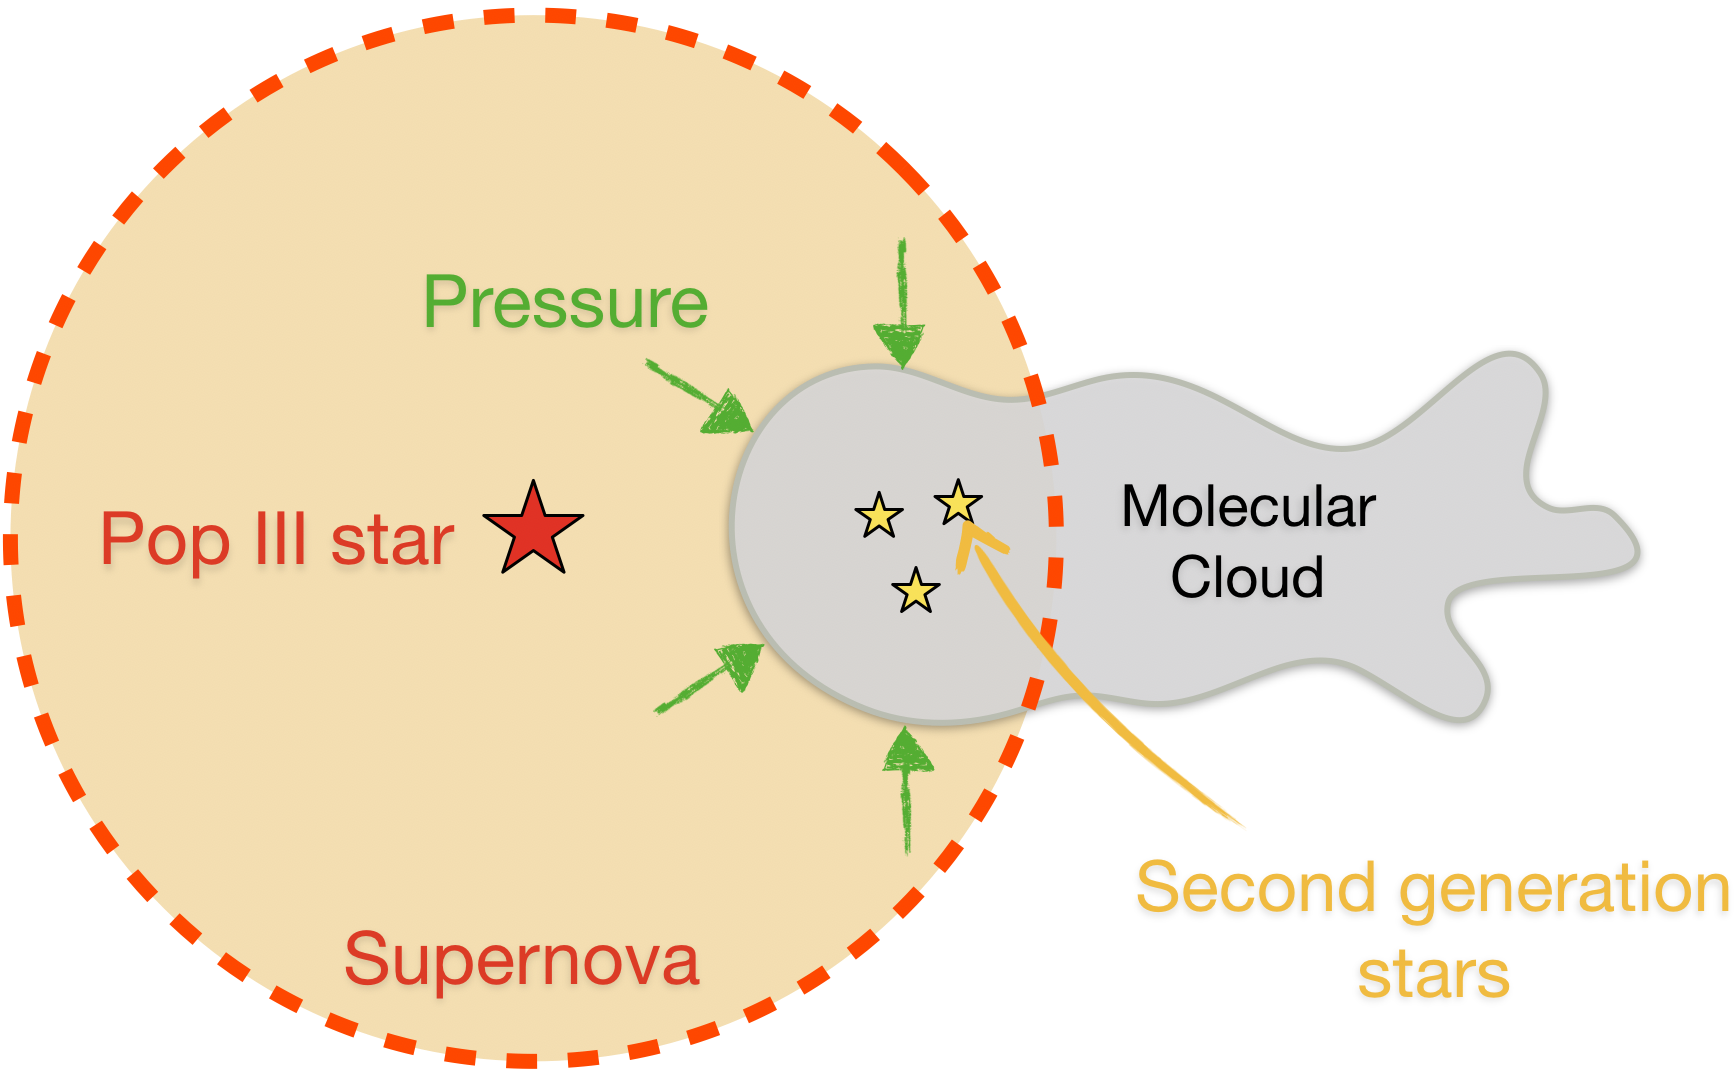
\includegraphics[width=0.6\textwidth]{figures/tsf2}
  \caption{Diagram of the triggered star formation scenario.}
  \label{fig:tsf}
\end{figure}

\textbf{Research plan:} We will study triggered star formation and its role in the formation of metal-poor stars using numerical hydrodynamic simulations with radiative feedback. These simulations will be run with Enzo: an adaptive mesh refinement (AMR) code for astrophysics \citep{Bryan2014}. Enzo is an excellent code to use because it solves the ideal magneto-hydrodynamic equations for the gas density, energy, and momentum, and magnetic fields, while also simulating the effects of stellar radiation feedback, and radiative cooling. Enzo is also integrated with the Grackle chemistry and cooling library \citep{Smith2017}, which will allow us to model the formation and destruction of $H_2$, as well as many other chemical species that affect the heating and cooling rates of the chemically-enriched gas. All of these processes are important to accurately model star formation in a physically realistic manner. 

By systematically studying triggered star formation, we can determine the conditions necessary for this to occur in the early universe, and most importantly, identify a causal link between the mass and yields of individual progenitor Pop III stars and the observable properties of their metal-poor descendants. We will run many realizations of these simulations spanning a parameter space consisting of the mass of the progenitor, the explosion energy, the mass of the molecular cloud, and the distance between the cloud and progenitor. By simulating a large parameter space, we can determine the optimal conditions that would allow this formation channel to occur. From these results, we can easily verify our claim that triggered star formation occurs on a shorter timescale than typical internal enrichment. The most important part of this project will involve a detailed study of how the metals from the supernova remnant mix into the cloud, which will determine the metallicity of the second-generation stars.

\textbf{Feasibility and previous work:} Multiple studies have shown that triggered star formation via cloud crushing is possible under certain conditions (\cite{Melioli2006}, \cite{Leao2009}), though none have specifically investigated the transfer of metals into the star-forming region. We can, however, gain useful insight from these existing simulations. \cite{Melioli2006} analytically determined when triggered star formation can occur in the parameter space of supernova radius and cloud density. They confirmed their results with hydrodynamical simulations. We will use these results as a guide for constructing our parameter space, but also test cases that would, according to their model, not induce star formation. Not only will this test the robustness and reproducibility of their results, but it may also reveal important differences that could arise from different simulation codes, grid resolutions, cooling models, and explosion energies.

\textbf{Analysis:} We will track the gravitational collapse -- or lack thereof -- and determine when star formation occurs by performing various analyses in post-processing. The simplest way to approximately determine when the cloud becomes gravitationally unstable is to measure the ratio of the enclosed mass to the Bonnor-Ebert (BE) mass. It is important to use the BE mass, rather than the Jeans mass because the hot supernova remnant will provide external pressure on the cool molecular cloud. This pressure acts to decrease the critical mass necessary for gravitational collapse leading to the formation of stars.

With each of our triggered star formation simulations, we will analyze the metal transport from the supernova remnant into the cloud, to determine the metallicity of the second-generation stars. We will investigate how the distribution of metallicity vs density and radius evolves over time. Once the mixing timescale becomes longer than the free-fall time of the cloud, metals will no longer efficiently mix into the core, and thus, this will determine the resultant metallicity of the subsequent stars. 

\textbf{Outcome:} If metals do not efficiently mix into the cloud, this could potentially explain how the low metallicity, CEMP-no stars in Group III formed, and allow us to estimate the properties of their progenitors. If metals mix in more efficiently, this could potentially explain the origin of the higher metallicity CEMP-no stars in Group II. Either way, if the conditions for triggered star formation can be achieved in the early universe, \textbf{these simulations will help explain the existence of the CEMP-no stars via a new formation channel.} These simulations will also provide a direct link between the properties of second-generation stars and \textit{individual} Pop III progenitors. If and when we observe metal-poor stars formed by triggered star formation, the results of this work will allow us to determine the properties of the stars that created them.

%%% TSF FIGURE ORIGINAL PLACEMENT %%% 
%\begin{figure}
%  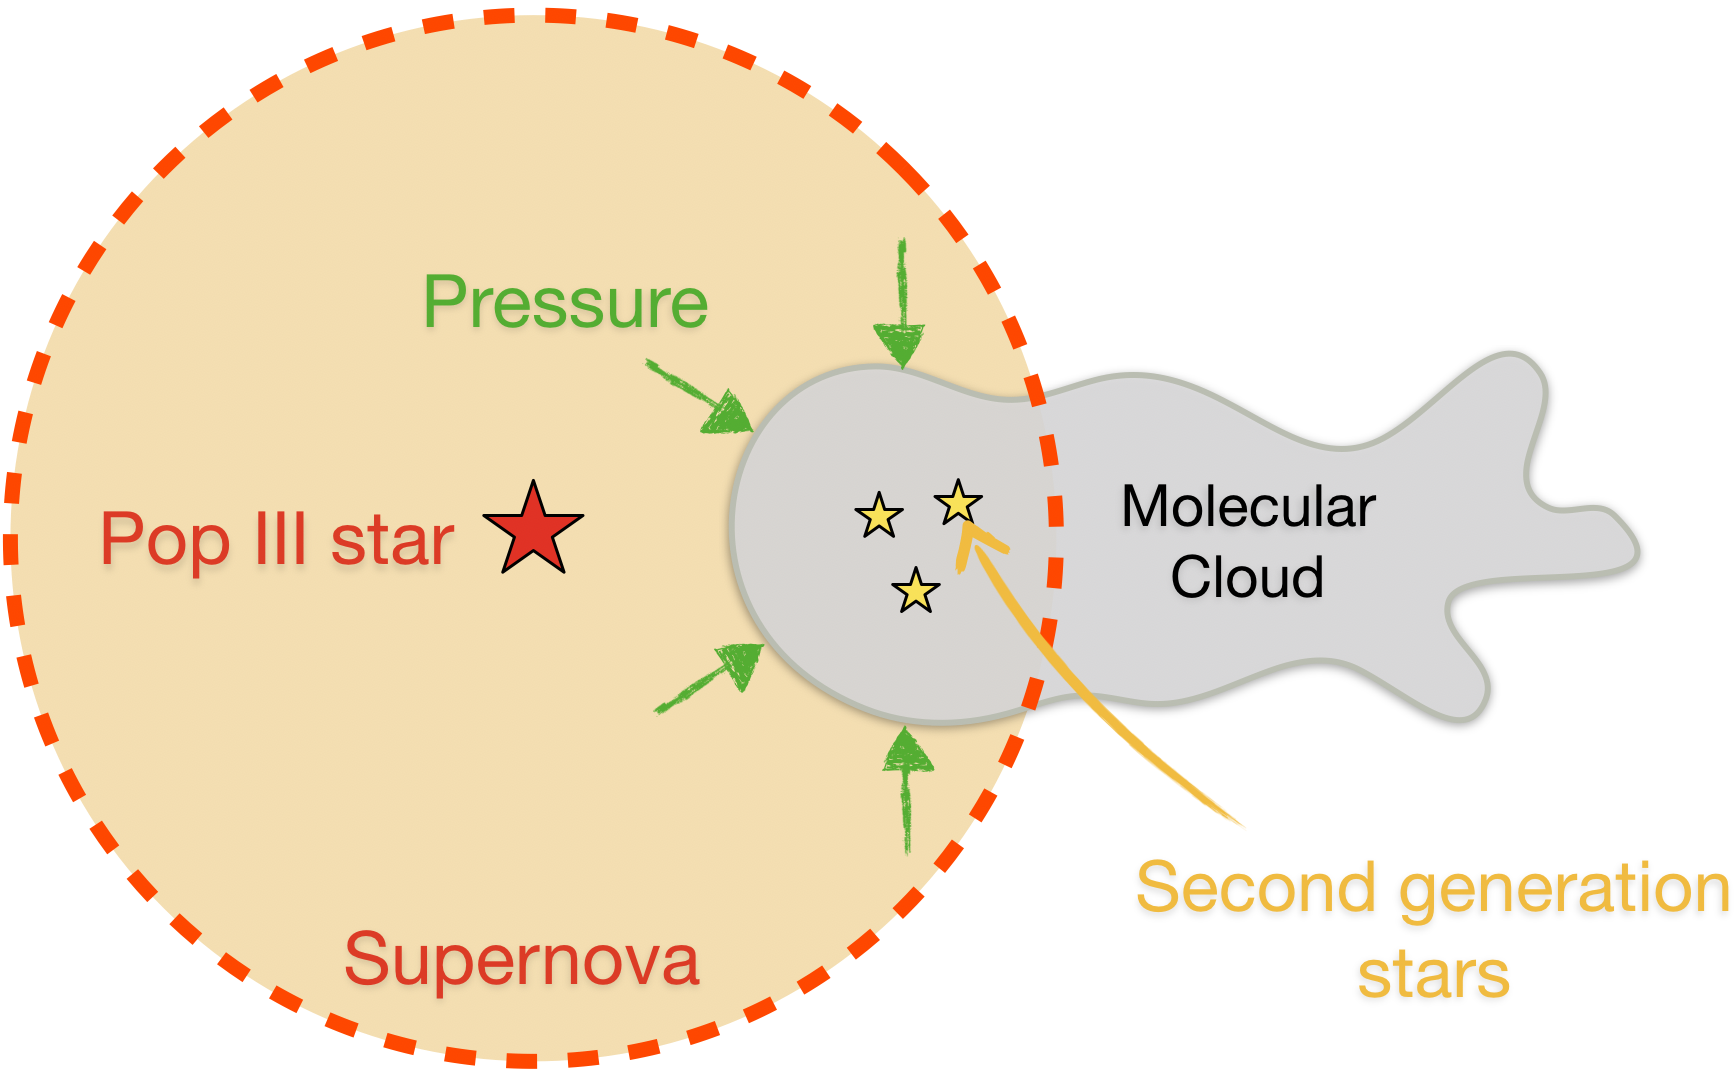
\includegraphics[width=0.6\textwidth]{figures/tsf2}
%  \caption{Diagram of the triggered star formation scenario.}
%  \label{fig:tsf}
%\end{figure}

While triggered star formation could produce Pop II stars enriched by a single progenitor, it is certainly not the only formation channel for metal-poor stars in the local universe. To better determine the properties of the first stars, we must also understand the metal enrichment and formation of second-generation stars enriched by multiple progenitors.

\subsection*{Project 2: Tracking Metals from Pop III Stars in Cosmological Simulations}
\label{subsec:tracer_particles}

\textbf{Goal:} With this project, we will, for the first time, provide a direct connection between multiple progenitors and their metal-poor descendants by tracking the metals from the supernovae of individual population III stars. Not only will this allow us to report \textit{exactly} how many Pop III stars enrich a given Pop II star cluster, we will also know the relative fractions that come from each progenitor. Since we will be able to tell the exact mass and metal yields of each Pop III star, we will be able to make predictions about the properties of the progenitors of the actual CEMP-no stars observed in the halo of our galaxy and in UFDGs. 

\textbf{Research plan:} To model the star formation process in a realistic, self-consistent manner, we will run a cosmological simulation initialized at a time before the formation of the first stars. The initial conditions for this simulation will be generated using MUSIC (Multi-scale initial conditions for cosmological simulations) \citep{Hahn2011}, using the most recent cosmological parameters obtained by \cite{Planck2018}. MUSIC allows us to initialize a simulation at high redshift, simulate a large, representative, volume of the universe, and then restart the simulation, "zooming-in" on particular subvolumes to more accurately resolve the formation of dark-matter halos where stars will form. These simulations will be run with Enzo for the reasons described in section \ref{sec:tsf}. Another benefit of this code is by using AMR we can focus the bulk of the computational resources on high-density dark matter halos and star-forming clouds.

However, in a cosmological simulation, resolving objects the size of individual stars is not computationally tenable. We, therefore, use a sub-grid model for stars and stellar feedback. Stars in the simulation are represented as point particles, advected in a Lagrangian manner, in contrast to the advection of the fluid fields which is done on an Eulerian grid. An important feature of these star particles is they inject energy and momentum back into the grid via heat and radiation pressure. The stars also produce ionizing Lyman-Werner radiation capable of dissociating $H_2$ molecules \citep{Safranek-Shrader2012}. The stars will continue their feedback until they've exhausted their time on the main sequence, at which point they produce a supernova. Unlike previous simulations of Pop III stars (e.g. \cite{Smith2015}, \cite{Chiaki2019}), we will vary the explosion energy depending on the mass of the progenitor. This allows us to simulate different types of explosions from faint supernovae to hypernovae, which produce different metal yields. The lifetimes of the Pop III stars will be determined from \cite{Schaerer2002} and the supernova metal yields will be taken from \cite{Nomoto2006}.

\begin{figure}
  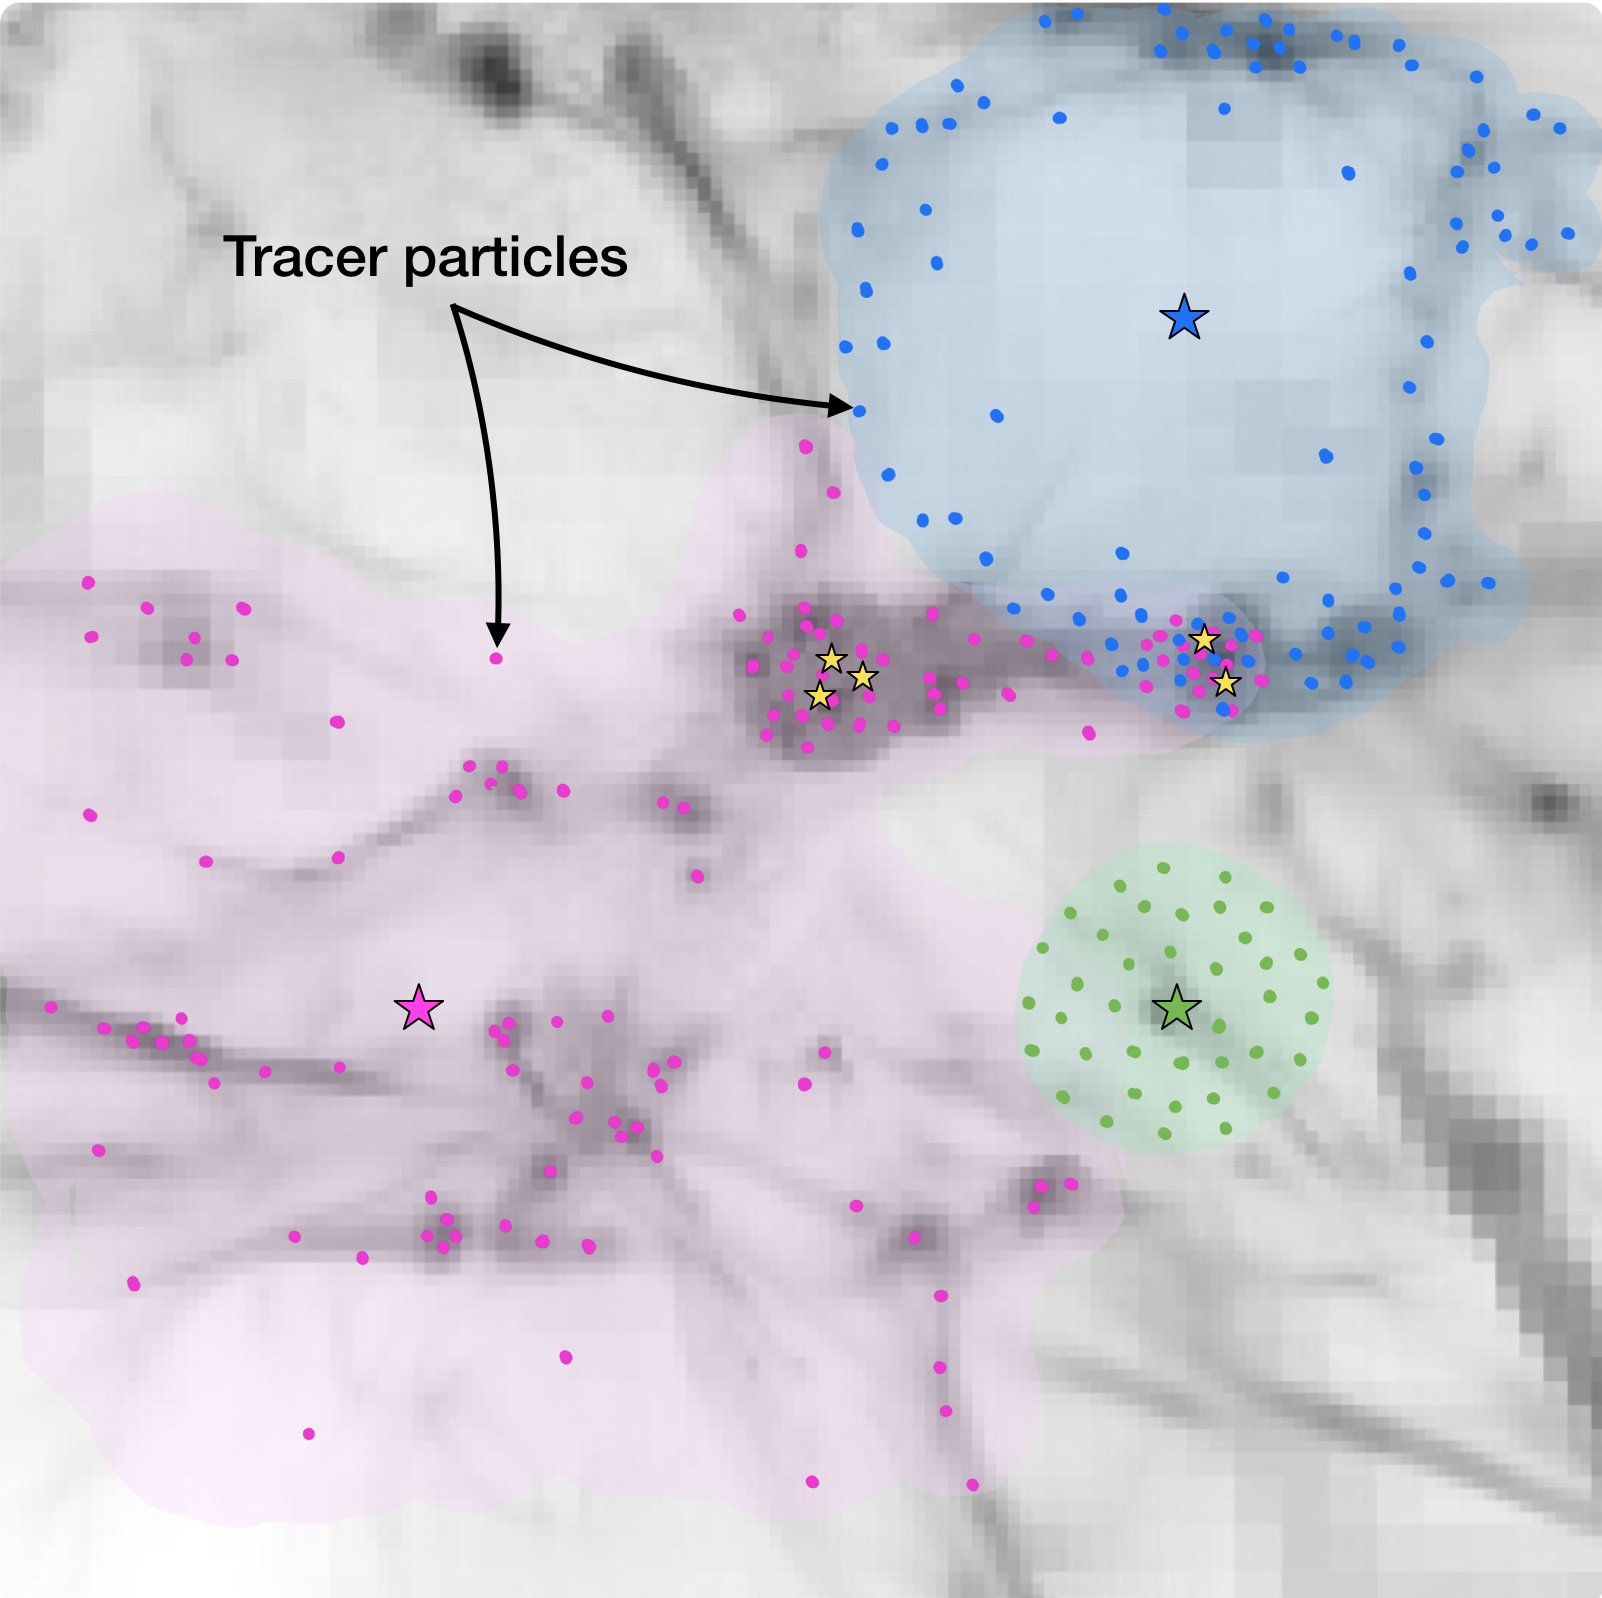
\includegraphics[width=0.6\textwidth]{figures/tracer_final}
  \caption{Qualitative illustration of metal tracer particles. Black and white colors represent gas density in an example cosmological simulation. Blue, pink, and green highlighted regions represent metal enrichment from the supernova remnants of Pop III stars (blue, pink and green stars). Colored points represent tracer particles. Gold stars represent potential sites of second-generation star formation. No stars are actually present in the example simulation.}
  \label{fig:tracer}    
\end{figure}

When the Pop III stars explode, energy, momentum, and metals are deposited onto the grid in a spherical region around the star. However, unlike any previous cosmology simulation involving chemical connection between Pop III stars and UFDG progenitors, we will inject tracer particles into the supernovae. These massless tracer particles will have identifiers unique to the Pop III star that produced them. They will be advected with the metals from the supernovae, and thus, will track the proliferation of the metals from their source. Over time, these particles will collapse with the metals into high-density regions where the second-generation stars will form. Due to the unique identifiers of the tracer particles, \textbf{we will be able to tell exactly which Pop III stars produce the metals that enrich the second-generation stars, and how many progenitors they have.} A qualitative illustration of this is shown in figure \ref{fig:tracer}. This is of great importance because it will provide a direct connection between the first and second stars. With a large enough sample of Pop III stars in the simulation, we will be able to make statistically significant conclusions about how often metal-poor stars are enriched by one or more progenitors and the fraction of metals coming from each. To ensure we have a sufficient number of dark matter halos and Pop III stars, we will choose a box size of 1 co-moving Mpc, a root grid resolution of $256^3$, with a maximum of 12 levels of refinement. This gives a minimum cell size of 0.1 proper pc. Given this simulation domain, we would expect on the order of 500 Pop III stars to form. For the sake of argument, if one assumes a second-generation star-forming region has, at most, 5 distinct progenitors, this leaves a minimum of 100 individual sites to investigate the formation of metal-poor stars.

\textbf{Outcome:} Not only will these simulations allow us to study the number of progenitors seeding the second stars, but they will also allow us to determine where the progenitors lived. Pop II stars are either enriched internally, by progenitors within the same halo, or externally by progenitors in a neighboring halo. Our tracer particles will show which of these channels occurs more frequently, and the differences in metal enrichment between the two scenarios. By including multiple types of supernova with different metal yields, we can determine how Group II and Group III CEMP-no stars are formed, and why there are two distinct groups.

%%% ORIGINAL PLACEMENT TRACER PARTICLES FIGURE %%%%
%\begin{figure}
%  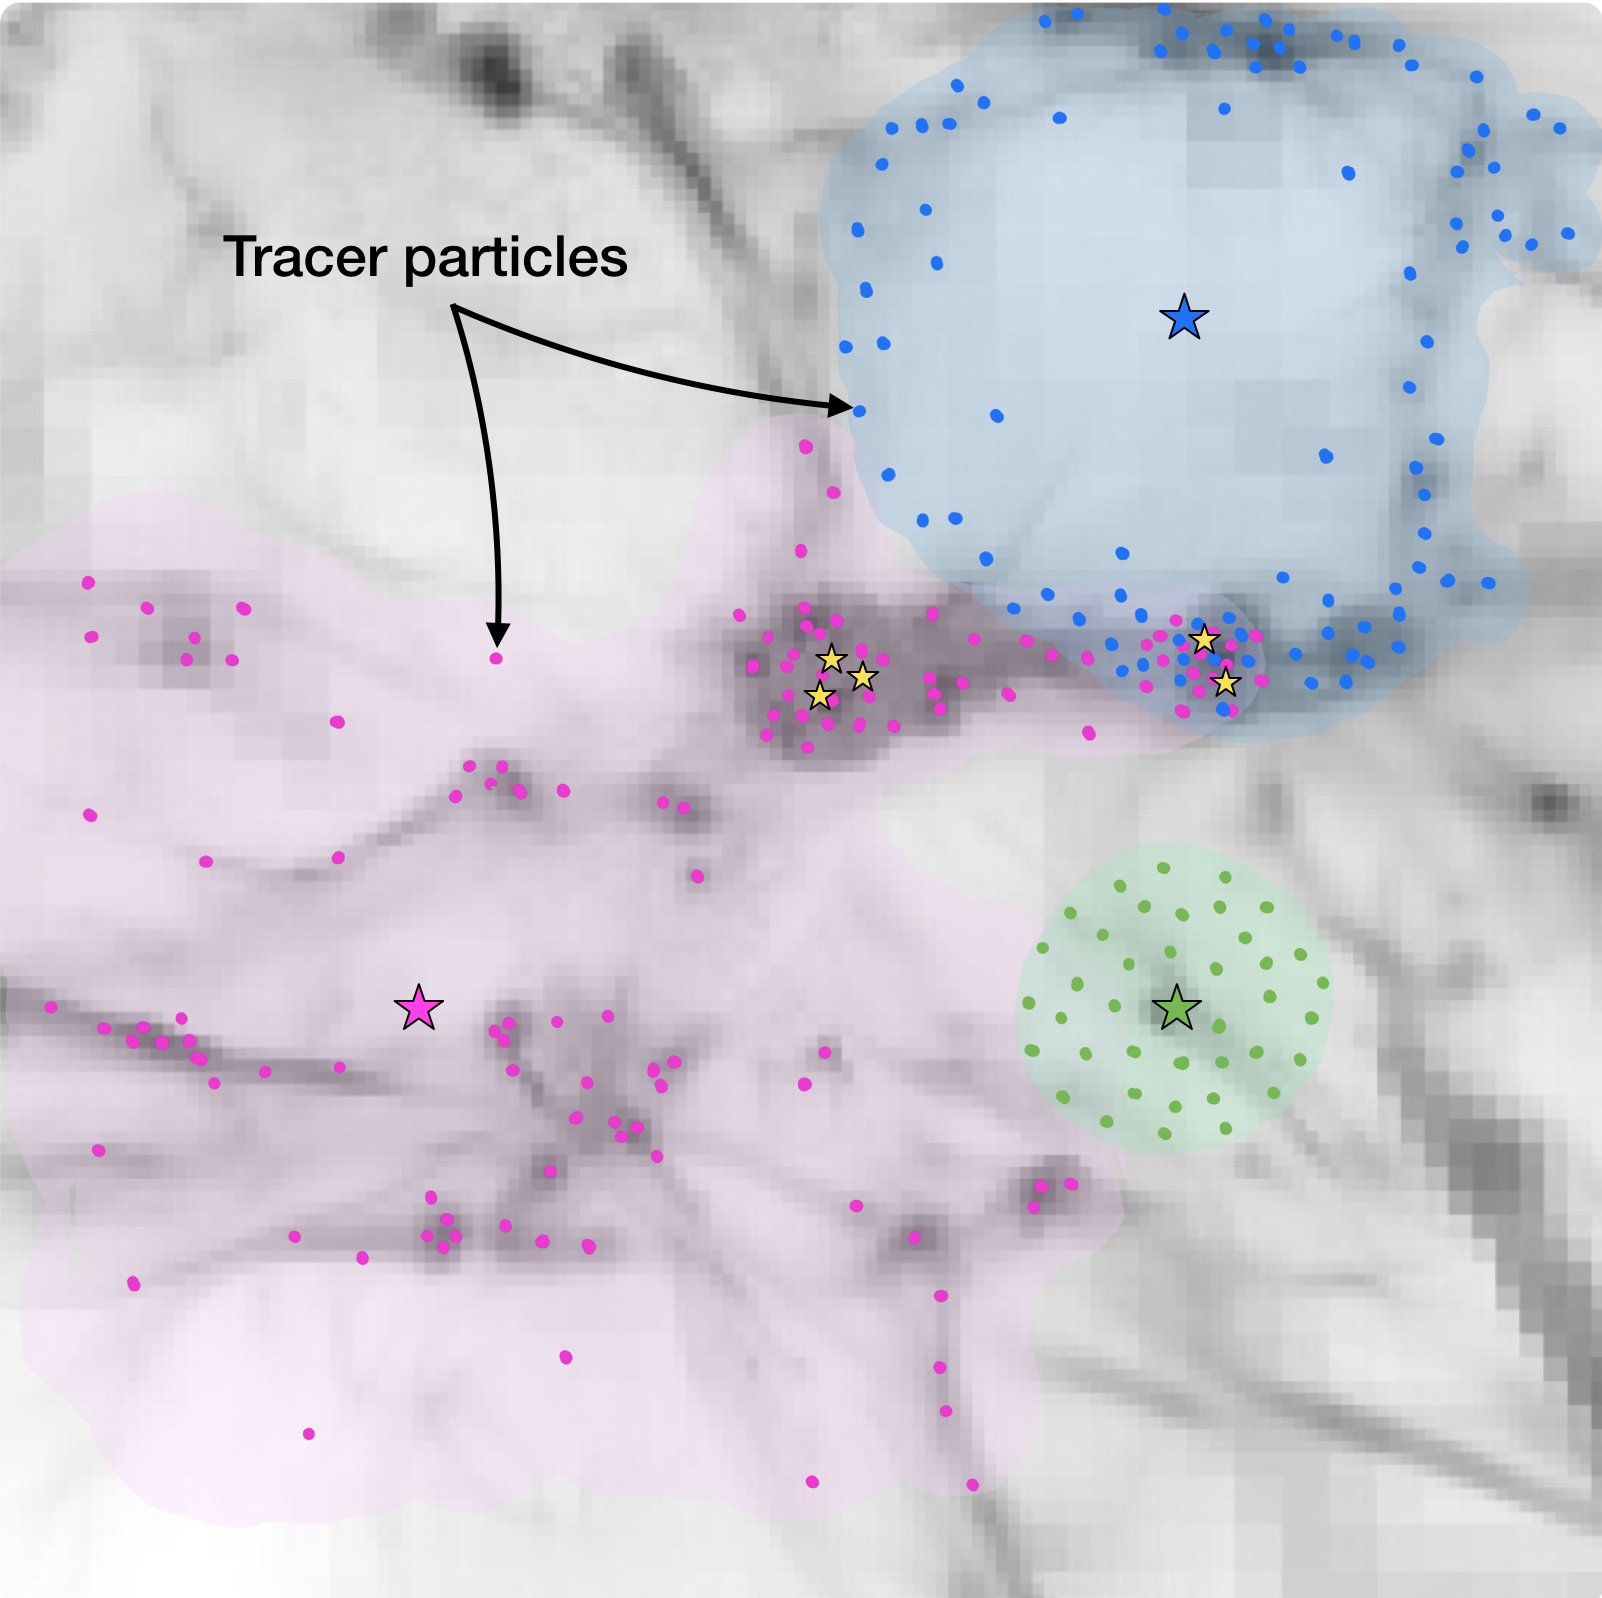
\includegraphics[width=0.6\textwidth]{figures/tracer_final}
%  \caption{Qualitative illustration of metal tracer particles. Black and white colors represent gas density in an example %cosmological simulation. Blue, pink, and green highlighted regions represent metal enrichment from the supernova remnants %of Pop III stars (blue, pink and green stars). Colored points represent tracer particles. Gold stars represent potential %sites of second-generation star formation. No stars are actually present in the example simulation.}
%  \label{fig:tracer}    
%\end{figure}


\subsection*{Access to Resources}

Our computational cosmology group has access to the PACE high-performance computing cluster at Georgia Tech, with 8 dedicated nodes, each with 28 cores, for our use only. We also have access to shared queues with 40,000 cores. These resources will be available to run our simulations and perform the necessary analyses. 

\subsection*{Relevance to NASA's Science Mission Directive}
Together, the two projects put forth in this proposal will address the question of how we can relate the properties of the second-generation stars with the first generation, Population III stars. Additionally, this work has the power to explain the different formation channels and conditions that lead to the origin of Group II and Group III CEMP-no stars. On a more fundamental level, our simulations will provide a deep connection between the metal-free universe and the one we see today, enriched by metals from the first stars. \textbf{Both of these projects are in direct alignment with NASA's Science Mission Directive for the "Cosmic Origins" section of the Astrophysics Research Program.} We share the same goals of discovering how stars form within galaxies; and discovering how these complex systems create and shape the structure and composition of the universe on all scales. Our cosmology simulations address these questions on the largest scales, and our triggered star formation simulations investigate these questions on smaller scales within individual galaxies. The timing of this research is optimal because our simulations and analysis will explicitly support NASA's future missions with the upcoming James Webb Space Telescope (JWST). JWST will be able to see deeper into the young, metal-poor universe than any previous telescope and study the environments in which the second-generation stars form. Our simulations will provide predictions for what JWST will see and aid in the interpretations of the observations. Specifically, we can make predictions about the metal content and distribution of galaxies in the early universe. Broadly speaking, since the first metals in the universe formed in the first stars, this research will bring us one step closer to understanding one of NASA's most fundamental questions, how did we get here?

\bibliography{proposal}
\end{document}
